\chapter{Results - Work in Progress}\label{chapter:results}
All experimental results are compiled into this chapter, starting with the optimization of the hyperparameters followed by the runtime and classification metrics of the object recognition tasks and finally the generalization experiments.
\section{Hyperparameters}
The 3 tuples of hyperparameters found for each neural network architecture that achieved the highest accuracy on the basic, non-perturbed version of the dataset are listed in the tables \ref{tab:pytorch-best} and \ref{tab:bindsnet-best}. They are found by refining the hypergrid around the most promising candidates after an initial extensive search. The best hyperparameter tuple is used in training and inference for the remainder of the experiments, unless explicitly mentioned otherwise.
\begin{table}[H]
\centering
\begin{tabular}{lllll}
\hline
model                  & batch size & learning rate & routing iterations & accuracy \\ \hline
matrix capsule network & 21         & $\num{9e-3}$  & 2                  & 88.96\%  \\
                       & 19         & $\num{1e-2}$  & 2                  & 84.72\%  \\
                       & 21         & $\num{3e-2}$  & 2                  & 79.25\%  \\
vector capsule network & 1          & $\num{2e-4}$  & 2                  & 90.82\%  \\
                       & 3          & $\num{3e-4}$  & 2                  & 87.24\%  \\

                       & 2          & $\num{3e-4}$  & 2                  & 83.69\%  \\
CNN                    & 130        & $\num{1e-5}$  & -                  & 85.23\%  \\
                       & 128        & $\num{1e-5}$  & -                  & 84.25\%  \\
                       & 131        & $\num{1e-5}$  & -                  & 83.90\%  \\ \hline
\end{tabular}
\caption[Top 3 results of the hyperparameter optimization for the matrix capsule, vector capsule and convolutional neural networks]{Top 3 results of the hyperparameter optimization for the matrix capsule, vector capsule and convolutional neural networks. The highest classification accuracy on the test set is reached by a vector capsule network, closely followed by the best result of the matrix capsule network. Most of the top results of the vector capsules use very small mini batches or process single samples even, whereas the matrix capsules and CNN prefer mini batches one or two orders of magnitude larger respectively. No large variation ($\ll\cross 10$) in the range of preferred learning rate can be observed for any of the 3 networks. Note that routing does not apply to CNN training, vector capsules perform best at 2 iterations and matrix capsules only converge for a maximum of 2 iterations.}
\label{tab:pytorch-best}
\end{table}
\begin{table}[H]
\centering
\begin{tabular}{@{}lllllll@{}}
\toprule
hidden neurons & time & learning rate & decay rate & patience & interval & accuracy \\ \midrule
100            & 15   & $\num{5e-3}$  & 0.7        & 10       & 250      & 79.77\%  \\
100            & 5    & $\num{5e-3}$  & 0.7        & 10       & 250      & 78.04\%  \\
250            & 15    & $\num{7e-3}$  & 0.5        & 10       & 250      & 77.72\%  \\ \bottomrule
\end{tabular}
\caption[Top 3 results of the hyperparameter optimization for the spiking neural network]{Top 3 results of the hyperparameter optimization for the spiking neural network. The preferred tuples show only little variance and are confined to a small subspace of the hypercube. A smaller number of neurons in the hidden layer (search range from 25--1000) is clearly preferred by the network.}
\label{tab:bindsnet-best}
\end{table}\noindent
To visualize the distribution of the hyperparameters, each parameter's correlation with the accuracy is determined by computing the mutual information (MI) between the two distributions \cite{kraskov2004estimating}. The accuracy is plotted over the two parameters with the highest MI scores in figure \ref{fig:hyperparameters}.
\begin{figure}[H]
    \centering
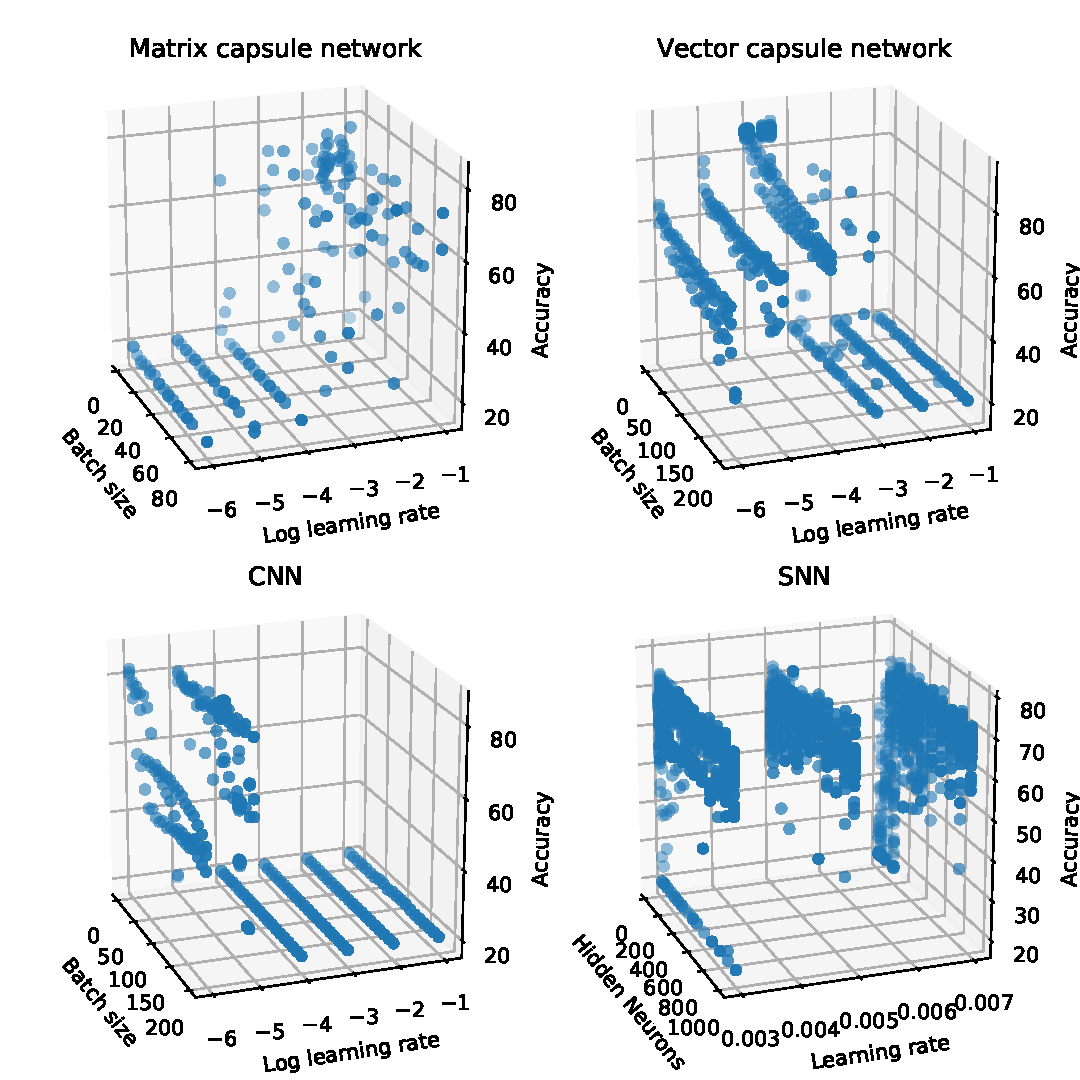
\includegraphics[clip,trim=0 0 0 .65cm,width=.79\textwidth]{figures/hyperparameters.pdf}
\caption[Accuracy over the two most relevant hyperparameters for each network]{Accuracy over the two most relevant hyperparameters for each network. The CNN and especially the vector capsule network highly correlate with batch size, while the SNN and the matrix capsule network in particular show considerable variance of accuracy along the axes.}\label{fig:hyperparameters}
\end{figure}\noindent
The temporal progression of training is investigated by plotting accuracy on the test set after each training epoch for the top 3 hyperparameter tuples of each network architecture (cf. figure \ref{fig:learning-curves}).
\begin{figure}[H]
    \centering
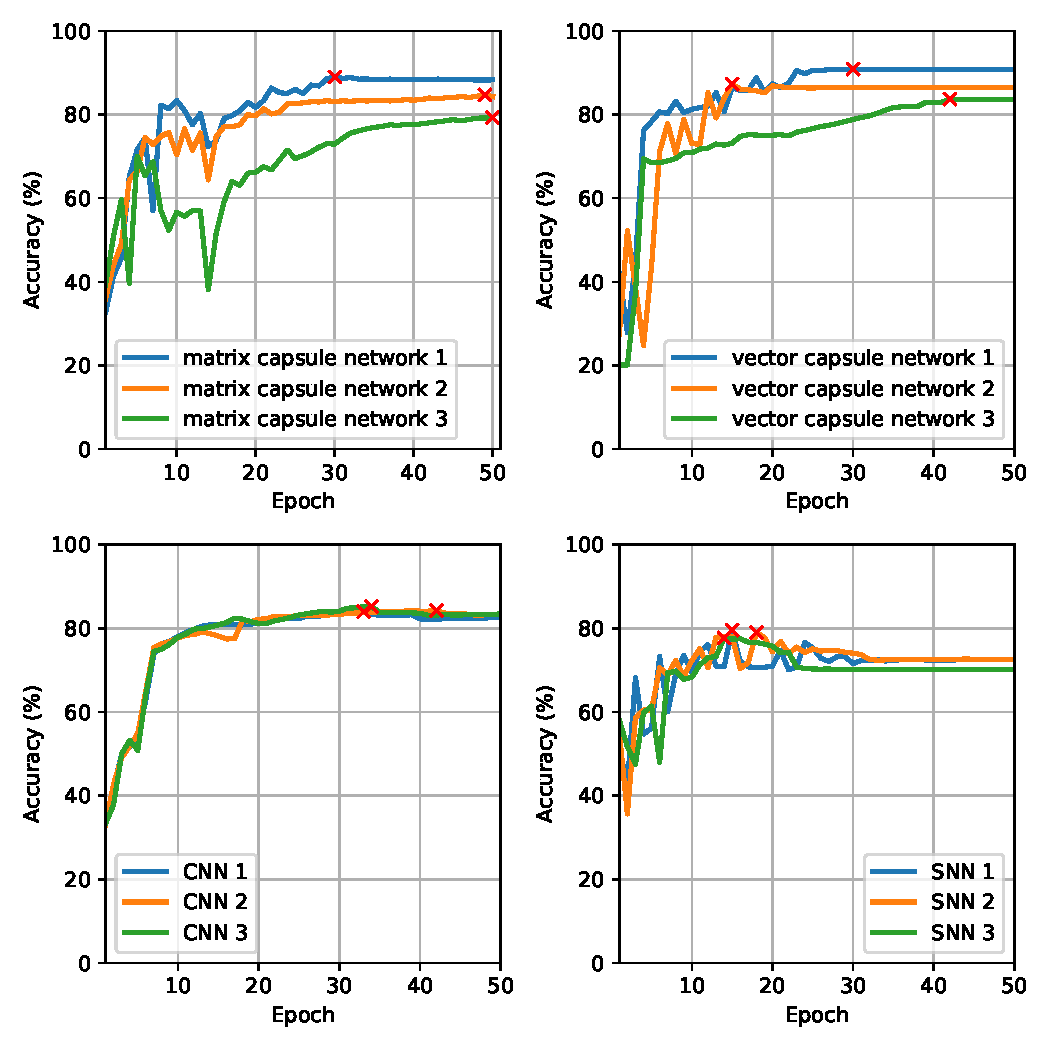
\includegraphics[width=\textwidth]{figures/learning_curves.pdf}
\caption[Accuracy on the test set during training over 50 epochs for all network architectures]{Accuracy on the test set during training over 50 epochs for the top 3 hyperparameter tuples of all network architectures. The red cross marks the epoch with the highest accuracy for each configuration. The capsule networks only start learning after several epochs and keep zigzagging for several more. Of all the architectures, CNNs show the most stable behavior and converge straightforwardly while the SNNs show somewhat unstable behavior before they converge. Additionally, the SNNs reach their maximums before convergence and lose a few percentage points before they converge.}\label{fig:learning-curves}
\end{figure}\newpage\noindent
\section{Runtime}
Figure \ref{fig:memory} shows the memory usage of each network required to train and test a single input image at $32\cross 32$ pixels. This is contrasted with the number of trainable parameters. There is a huge difference in the required memory on GPU. The networks based on capsules can easily take up several GB of memory, whereas the CNNs and SNNs use less than 100 MB. The exact numerical results are also available in table \ref{tab:memory}.
\begin{figure}[H]
    \centering
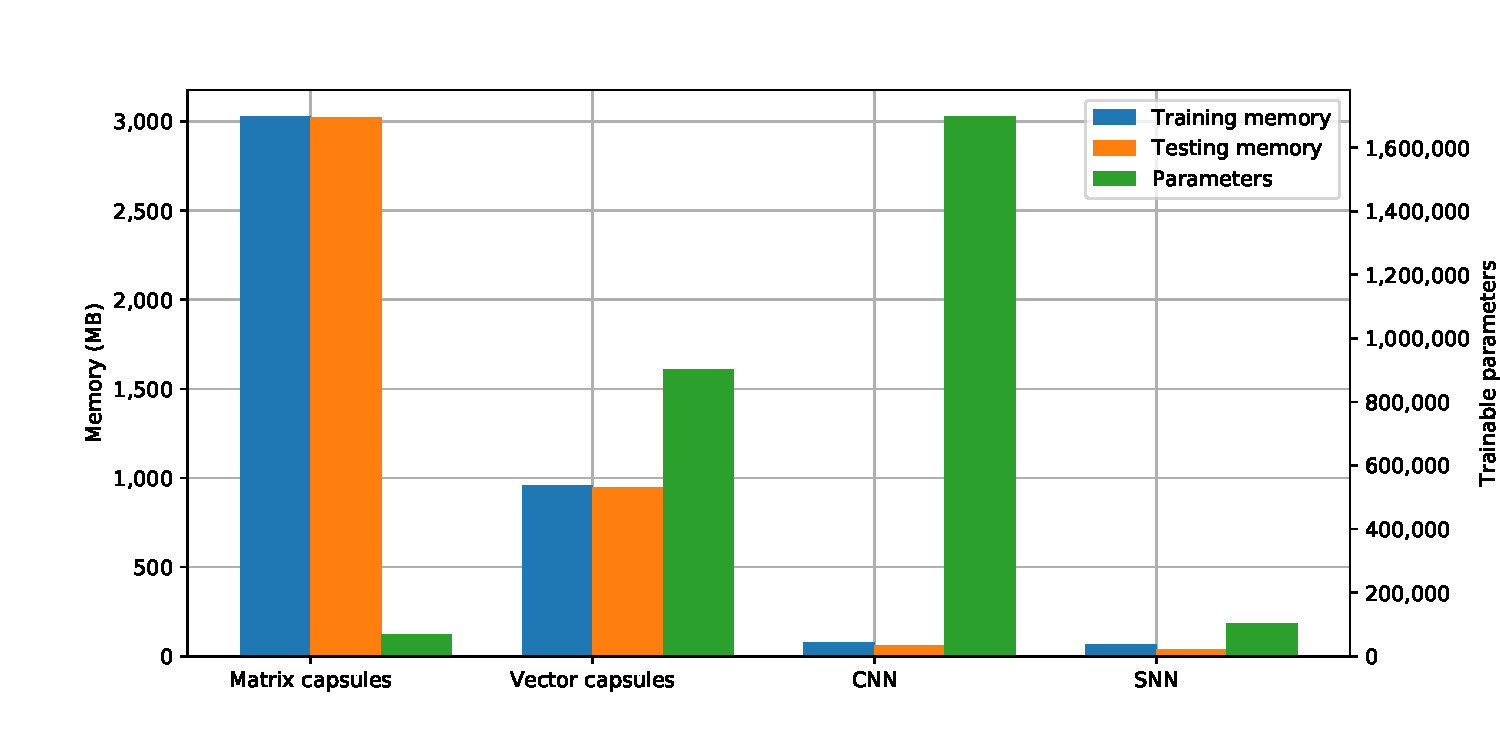
\includegraphics[clip,trim=1.5cm 0 0 0,width=\textwidth]{figures/memory.pdf}
\caption[Memory requirements and number of trainable parameters for all the networks]{Memory requirements and number of trainable parameters for all the network architectures. The matrix capsules require the most memory by far but they also need to train the fewest parameters to learn the data. They are closely followed by the SNN regarding number of parameters while the CNN and vector capsule network need many more parameters. SNNs are the only architecture that require both little memory as well as few parameters.}\label{fig:memory}
\end{figure}\noindent
% Please add the following required packages to your document preamble:
% \usepackage{booktabs}
\begin{table}[htp!]
\centering
\begin{tabular}{@{}lrrrr@{}}
\toprule
                     & Matrix capsules & Vector capsules & CNN             & SNN            \\ \midrule
Training memory (MB)      & $\num{3025.47}$        & $\num{956.16}$         & $\num{76.94}$   & $\num{64.29}$  \\
Testing memory (MB)       & $\num{3023.48}$        & $\num{945.76}$         & $\num{57.52}$   & $\num{38.46}$  \\
Trainable Parameters & $\num{67442}$          & $\num{901536}$         & $\num{1696645}$ & $\num{103005}$ \\ \bottomrule
\end{tabular}
\caption[Numerical results of the memory requirements and number of trainable parameters for all the networks]{Numerical results of the memory requirements and number of trainable parameters for all the networks. Note that the difference in memory requirements between training and inference is largest for the SNN, in both relative and absolute terms.}
\label{tab:memory}
\end{table}\newpage\noindent
For the final runtime metric, the actual time it takes to run through a training and inference epoch respectively is measured. Because of the uneven train/test set split, these measurements are additionally normalized over sample size. The measurements given in figure \ref{fig:runtime} therefore represent the average time it takes to process a single sample.
\begin{figure}[H]
    \centering
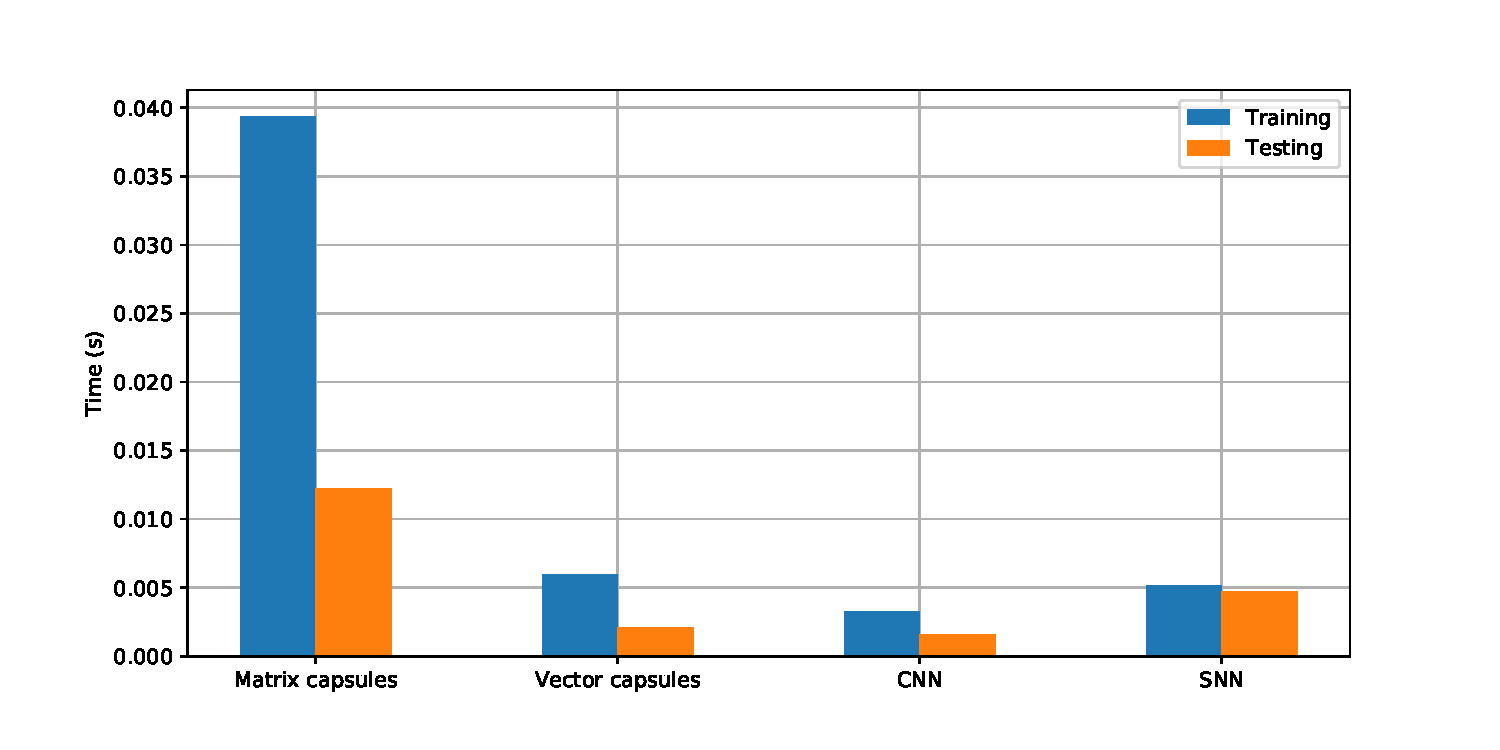
\includegraphics[clip,trim=1.3cm 0 2.5cm 1cm,width=\textwidth]{figures/runtime.pdf}
\caption[Training and inference runtime normalized over sample size]{Training and inference runtime normalized over sample size. All the network architectures with the exception of SNNs show a marked decrease in runtime for inference compared to training. This is particularly true for the matrix capsule network, which also has the longest absolute runtimes by a large margin.}\label{fig:runtime}
\end{figure}\noindent
To consider the advantage of highly parallel computing on GPUs all the runtime metrics are again measured during inference with the maximum possible mini batch size (cf. table \ref{tab:runtime}). 
% Please add the following required packages to your document preamble:
% \usepackage{booktabs}
\begin{table}[H]
\centering
\begin{tabular}{@{}lrrr@{}}
\toprule
                 & Matrix capsule network & Vector capsule network & CNN                   \\ \midrule
Time             & $\SI{0.0023}{\second}$   & $\SI{0.00025}{\second}$    & $\SI{0.00013}{\second}$ \\
Batch size       & $\num{465}$            & $\num{1897}$           & $\num{2406}$          \\
Memory footprint & $\SI{5492}{\mega\byte}$         & $\SI{6985}{\mega\byte}$         & $\SI{486}{\mega\byte}$         \\ \bottomrule
\end{tabular}
\caption[Runtime metrics for inference on GPU with maximally sized mini batches]{Runtime metrics for inference on GPU with maximally sized mini batches. The given time is the average per processed sample, whereas the memory footprint is for the entire mini batch. Note that the CNN can process the entire dataset in a single step without running into memory limitations.}
\label{tab:runtime}
\end{table}
\section{Object Recognition}
The object recognition task in these experiments consists of classifying images of 5 different classes. Each class is represented by 8 different instances viewed from roughly 160 different viewpoints. The networks are trained on 5 object instances of each class and then tested on the remaining 3. This means that an accuracy of $\SI{20}{\percent}$ is the worst possible score for a classifier -- a random guess without any learned knowledge. The classification metrics are compiled into confusion matrices and receiver operating characteristic curves for all the network architectures. The diagonal elements of the confusion matrix count the number of correct classifications for each object class, while the off-diagonal elements all correspond to misclassifications. ROC curves on the other hand allow a quick estimation at what cost (in the sense of false positives) classification accuracy is achieved. Summaries of the results for each network can be found in table \ref{tab:ranking} as well as figures \ref{fig:all-roc}, \ref{fig:roc-matrix}, \ref{fig:roc-vector}, \ref{fig:roc-cnn} and \ref{fig:roc-snn} on the following pages.
\begin{table}[H]
\centering
\begin{tabular}{@{}lllll@{}}
\toprule
Model    & Vector capsule network & Matrix capsule network & CNN                    & SNN                    \\ \midrule
Accuracy & $\SI{90.82}{\percent}$ & $\SI{88.96}{\percent}$ & $\SI{85.23}{\percent}$ & $\SI{79.77}{\percent}$ \\ \bottomrule
\end{tabular}
\caption[Ranking of the neural networks by their performance in object recognition]{Ranking of the neural networks by their performance in object recognition.}
\label{tab:ranking}
\end{table}\noindent
\begin{figure}[H]
    \centering
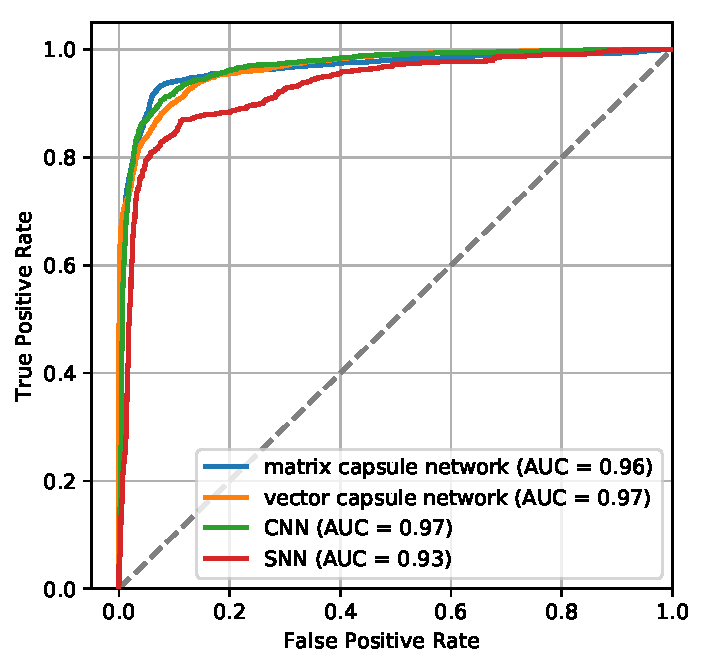
\includegraphics[width=.59\textwidth]{figures/all-roc.pdf}
\caption[Averaged ROC curves and AUCs for all the network]{Averaged ROC curves and AUCs for all the networks. The average curves are computed form the binary single-class ROC curves of each class. Note that all the networks offer a similar trade-off between cost and precision, except for the SNN, which cannot reach the same level of accuracy.}\label{fig:all-roc}
\end{figure}\noindent
\begin{figure}[H]
    \centering
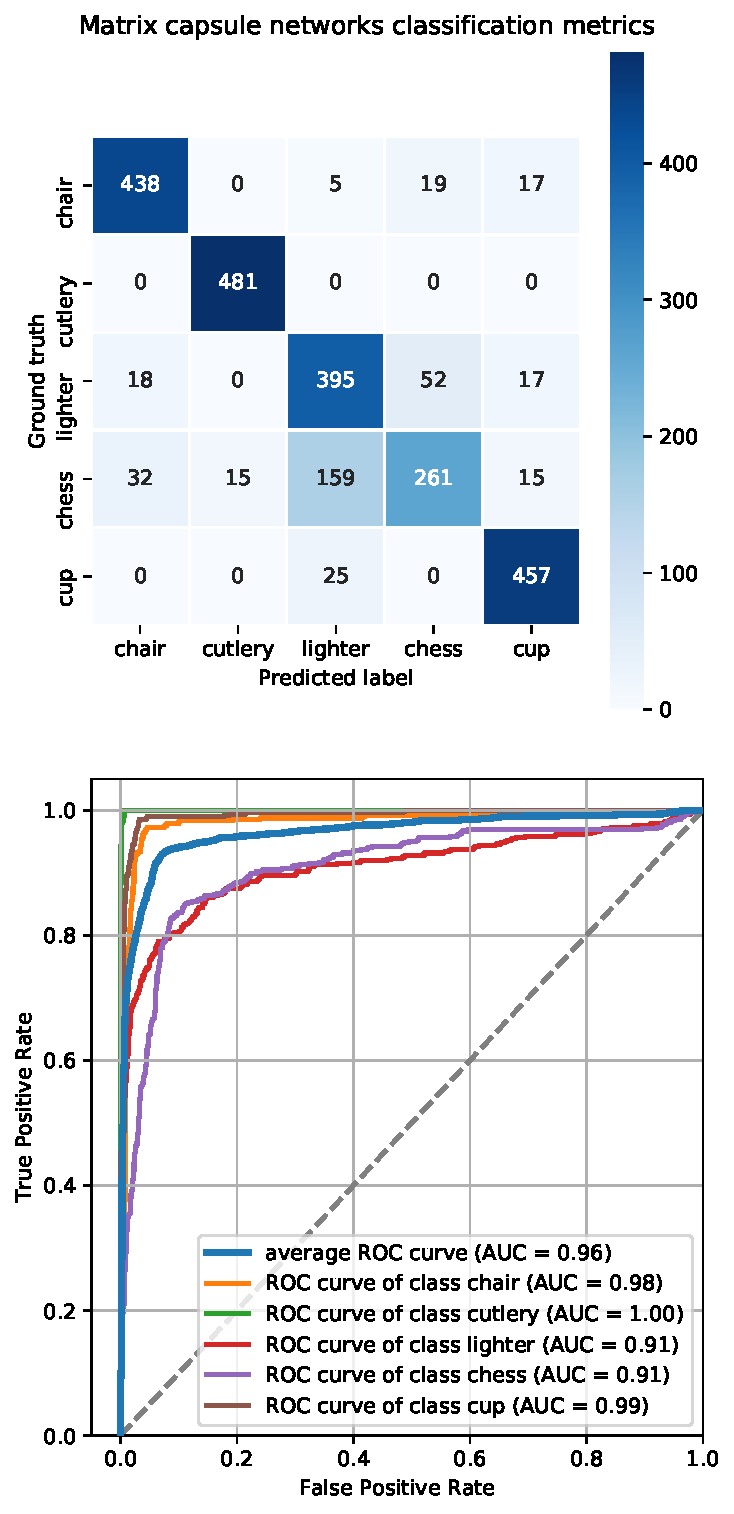
\includegraphics[width=.59\textwidth]{figures/roc_matrix.pdf}
\caption[Classification metrics for the matrix capsule network]{The network is best able to classify the object class of cutlery, never mistaking it for a different class. This is followed by the cups, although the network sometimes mistakes them for lighters. Most misclassifications happen for the chess objects, they are very often predicted to be lighters as well. The ROC curves on the right confirm this information. Classes chess and lighter perform below average, whereas the other curves approach a perfect classifier.}\label{fig:roc-matrix}
\end{figure}\noindent
\begin{figure}[H]
    \centering
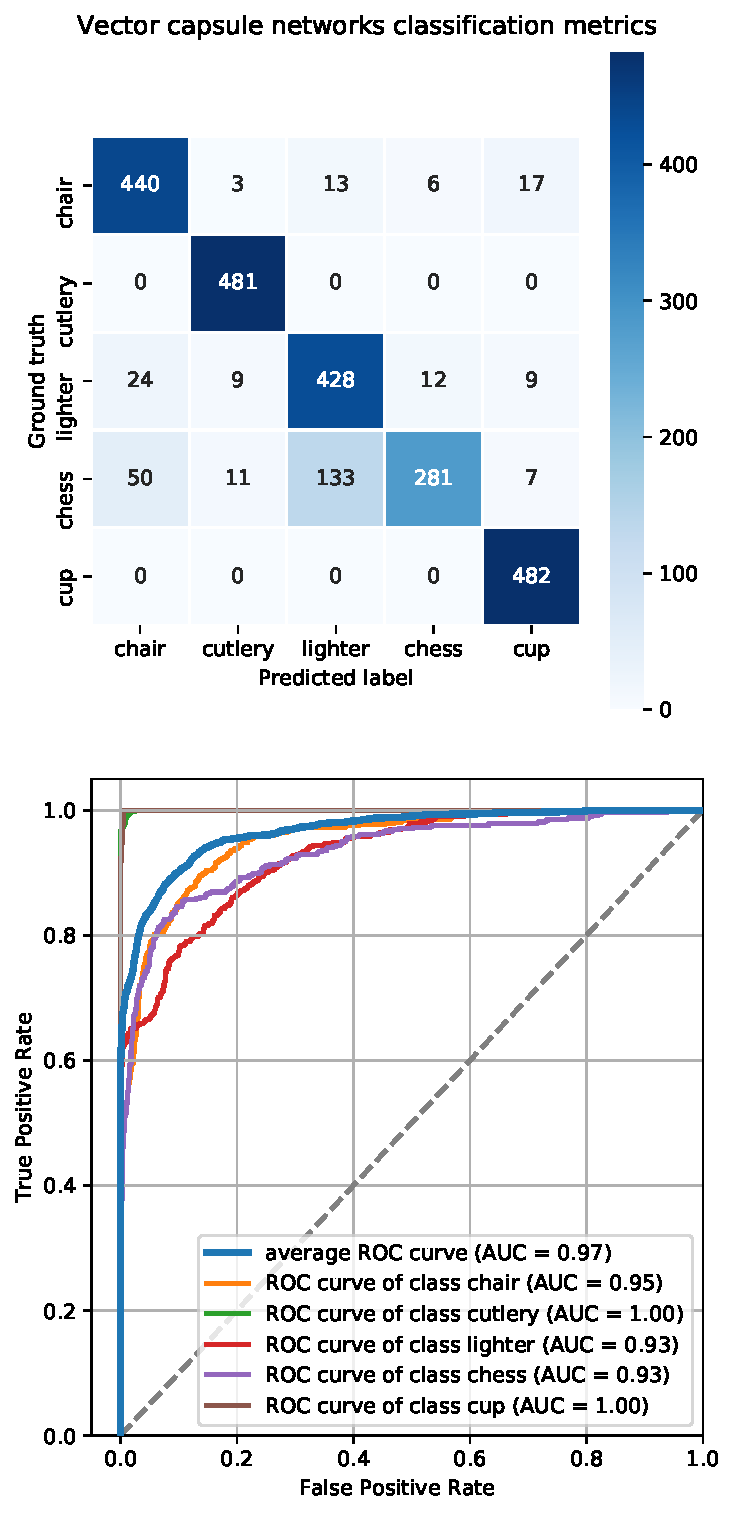
\includegraphics[width=.59\textwidth]{figures/roc_vector.pdf}
\caption[Classification metrics for the vector capsule network]{The network correctly identifies all the cutlery and cups without too many false positives, resulting in nearly perfect ROC curves for those classes. Like the matrix capsule network, it often mistakes objects of the chess class for lighters, although not quite as often as the matrix capsules do. On average the vector capsules outperform the matrix capsules by lowering the error rates of the lighter and chess classes as can be seen by the AUC. Performance on the other classes is either on par with matrix capsules or slightly reduced as in the case of the chairs (higher false positive rate).}\label{fig:roc-vector}
\end{figure}\newpage\noindent
\begin{figure}[H]
    \centering
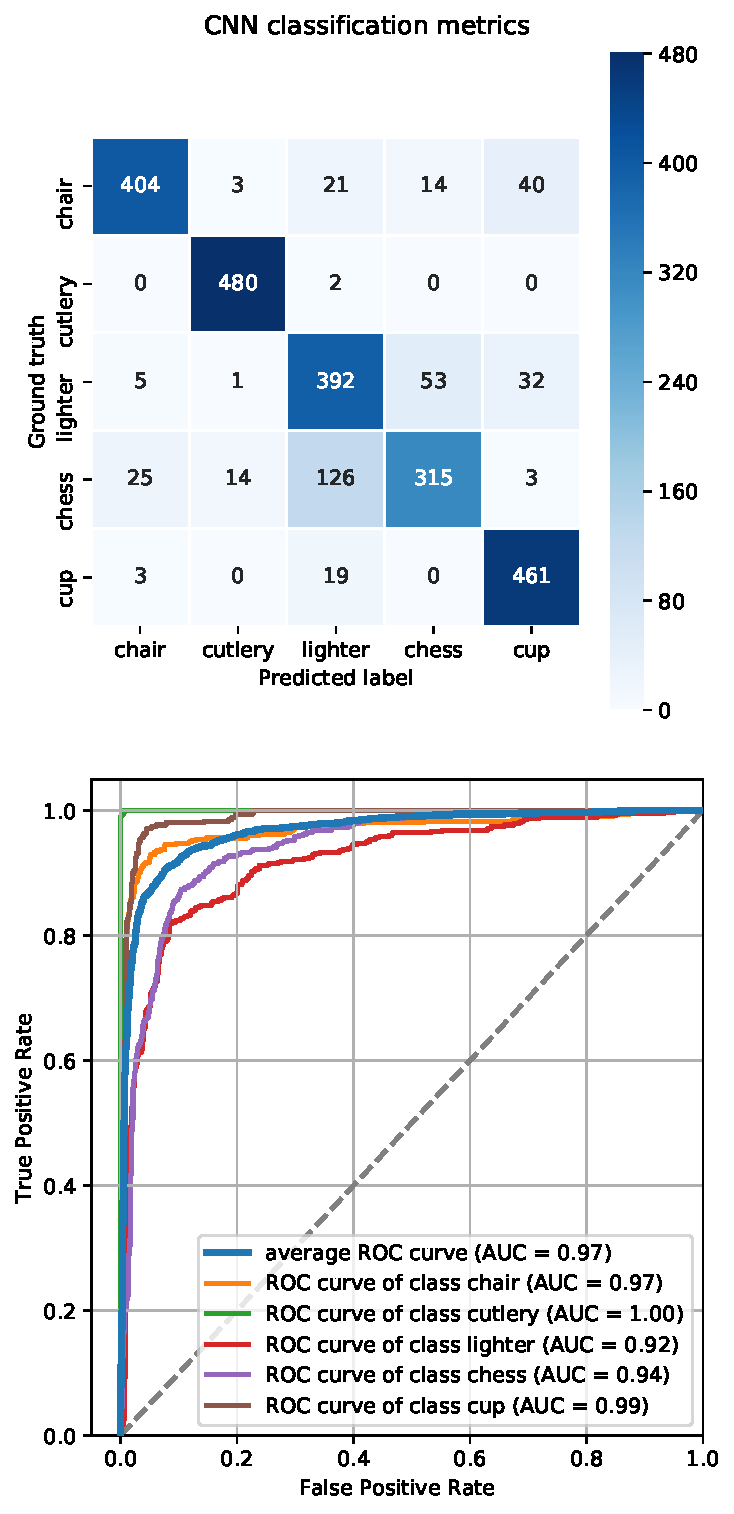
\includegraphics[width=.59\textwidth]{figures/roc_cnn.pdf}
\caption[Classification metrics for the CNN]{Classification metrics for the CNN. Similarly to the capsule networks, the CNN approaches a perfect classifier for the cutlery class and has problems keeping chess pieces and lighters apart. Additionally, the CNN outperforms the other networks when it comes to identifying chess pieces, even if it can't beat the capsule networks in accuracy across all the classes.}\label{fig:roc-cnn}
\end{figure}\noindent
\begin{figure}[H]
    \centering
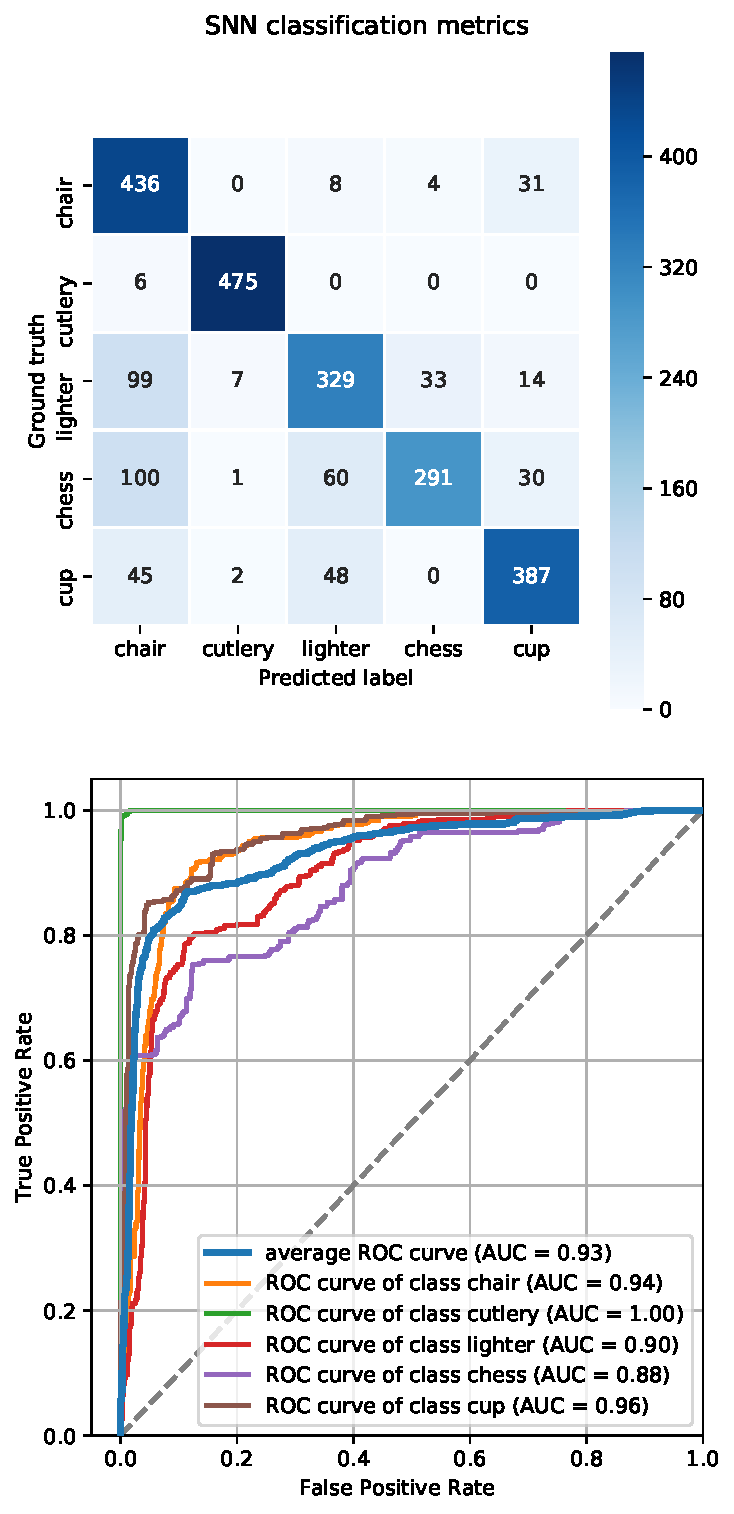
\includegraphics[width=.59\textwidth]{figures/roc_snn.pdf}
\caption[Classification metrics for the SNN]{Classification metrics for the SNN. The SNN shows the highest variance as can be seen by the off-diagonal elements in the confusion matrix and the distribution of ROC curves. In particular it often predicts a chair, except if it sees cutlery. On the other hand it does not nearly as often confuse chess pieces with lighters as the other networks.}\label{fig:roc-snn}
\end{figure}\noindent
\section{Generalization}
The networks trained on the basic object recognition dataset are tested against new variations in lighting. These variations in lighting include adding additional spot lights, changing intensity and position of the lights etc. Figure \ref{fig:lighting} shows the accuracy of each network during inference relative to the accuracy of the originally trained lighting. This is not the same as the perturbation parameterization used later as there are only three arbitrarily chosen light setups that do not cover the entire perturbation space. But it can be used as a baseline to determine, how useful that approach is.
\begin{figure}[H]
    \centering
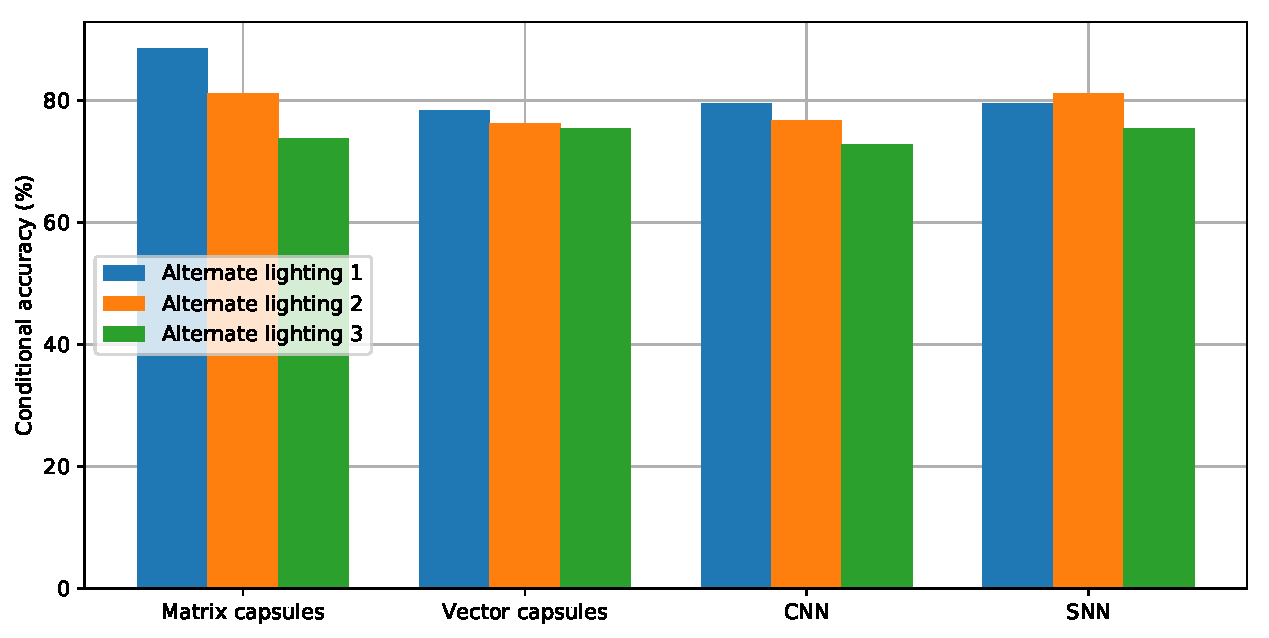
\includegraphics[width=\textwidth]{figures/lighting.pdf}
\caption[Relative accuracy under different lighting]{Relative accuracy under different lighting. The networks lose around $\SI{20}{\percent}$ of accuracy under unknown lighting. However, the matrix capsule network appears to have a small advantage over the other architectures as it reaches $\SI{80}{\percent}$ of its unperturbed accuracy on two of the three test sets.}\label{fig:lighting}
\end{figure}\noindent
The conditional accuracy used in these plots refers to the conditional probability of classifying an object correctly given perturbations. For the metrics, this can also be expressed as relative or conditional accuracy, i.e. accuracy on the perturbed data normalized over the unperturbed performance. Consequently a conditional accuracy of $\SI{100}{\percent}$ means the perturbation has no influence on classification accuracy. Robustness against perturbation or analogously the ability to generalize can then be interpreted as the conditional accuracy across the entire perturbation space (i.e. the area under the curve). The concept of generalization is explored further by measuring the AUC of the conditional accuracy for three kinds of perturbation. This is done by taking the optimized networks that were trained on the basic, unperturbed and unaugmented version of the object recognition dataset and test them on the perturbed versions, where the accuracy on each perturbed dataset corresponds to one measurement point.\newpage\noindent
The first perturbation is simple occlusion by geometric primitives placed on top of the object. Generating the perturbation in this ways makes it easy to sample from the distribution of the perturbation and compute an accurate curve and AUC (cf. figure \ref{fig:occlusion-generalization}).
\begin{figure}[H]
    \centering
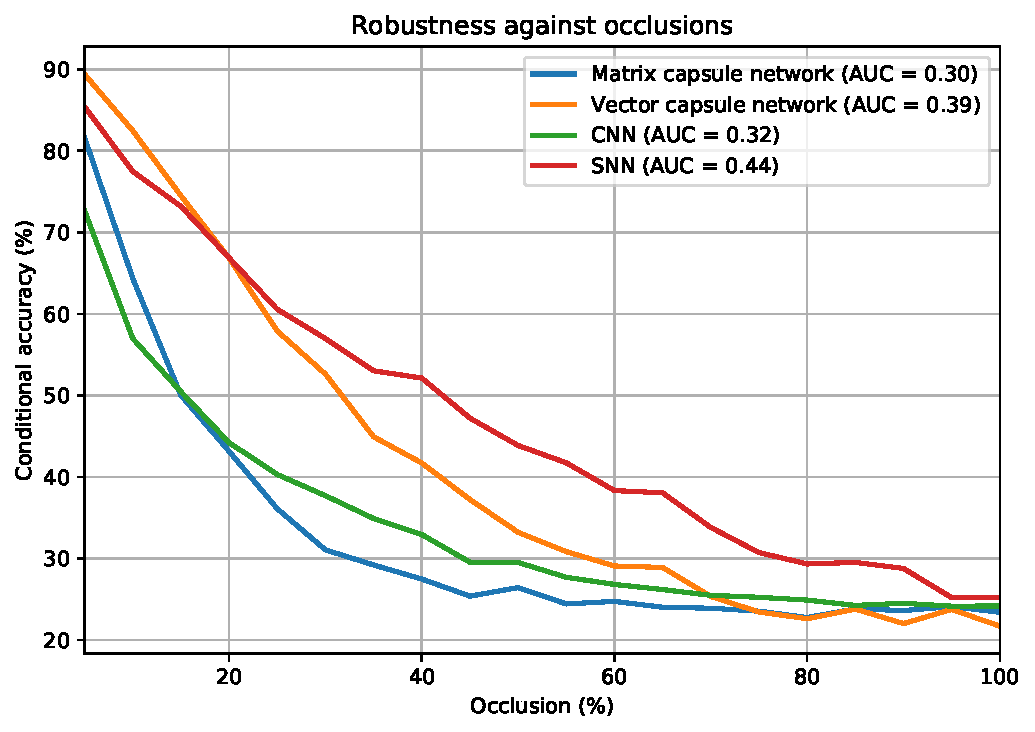
\includegraphics[width=\textwidth]{figures/occlusion.pdf}
\caption[Generalization of the networks in the presence of occlusion]{Generalization of the networks in the presence of occlusion. With increasing occlusion the networks' ability to classify goes down. Of all the networks, the SNN relinquishes the least accuracy by a large margin while the matrix capsule network shows the worst performance. Eventually, as the entire image is covered, all the classifiers perform randomly. Note that the accuracy curves occasionally cross each other}\label{fig:occlusion-generalization}
\end{figure}\noindent
Another interesting generalization ability is robustness against part-whole decomposition. A classifier that strictly adheres to part-whole relationships should not classify an object where those part-whole relationships have been deconstructed, i.e. they dont exist. The tile augmentation randomly switches image segments and therefore breaks relationships between features in pose space. By definition the robustness against part-whole decomposition is then the probability of the opposite event (i.e. misclassification). A perfectly generalizing classifier would therefore in the face of part-whole deconstruction give a random classification accuracy ($\SI{20}{\percent}$ in this experiment). The way this ability is defined may appear to measure the opposite of generalization but semantically this can be thought of as the ability to retain the coherence of internal representation against outside perturbation, i.e. generalization to novel situations. A plot of the curves and the networks' AUC can be found in figure \ref{fig:part-whole-generalization}.
\begin{figure}[H]
    \centering
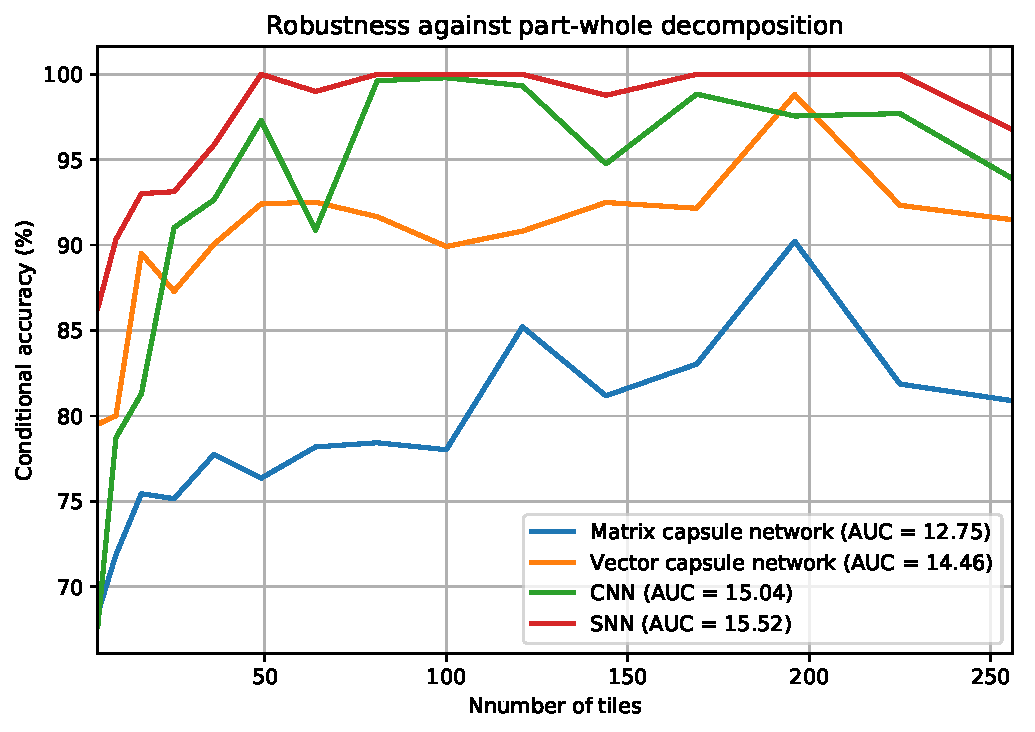
\includegraphics[width=\textwidth]{figures/part-whole.pdf}
\caption[Generalization of the networks in the presence of part-whole decomposition]{Generalization of the networks in the presence of part-whole decomposition. Again the matrix capsules show the least generalization, in thise case even by a large margin, almost across the entire perturbation space. The CNN generalized quite well and the SNN is again on top. Note that the number of tiles doesn't increase beyond 256. This is because the tiles eventually become smaller than $2\cross 2$ pixels and can no longer thought to include visually meaningful features.}\label{fig:part-whole-generalization}
\end{figure}\noindent
Finally, an attempt is made to determine the networks' ability to handle unknown viewpoints to classify known objects. To this end the networks are trained only on a subset of viewpoints whilst inference is performed on a test set including all the viewpoints. The relative amount of viewpoints to exclude from training is set incrementally for each measurement and randomly removed from the training set. The results of this endeavor may be observed in figure \ref{fig:viewpoint}.\newpage\noindent
\begin{figure}[H]
    \centering
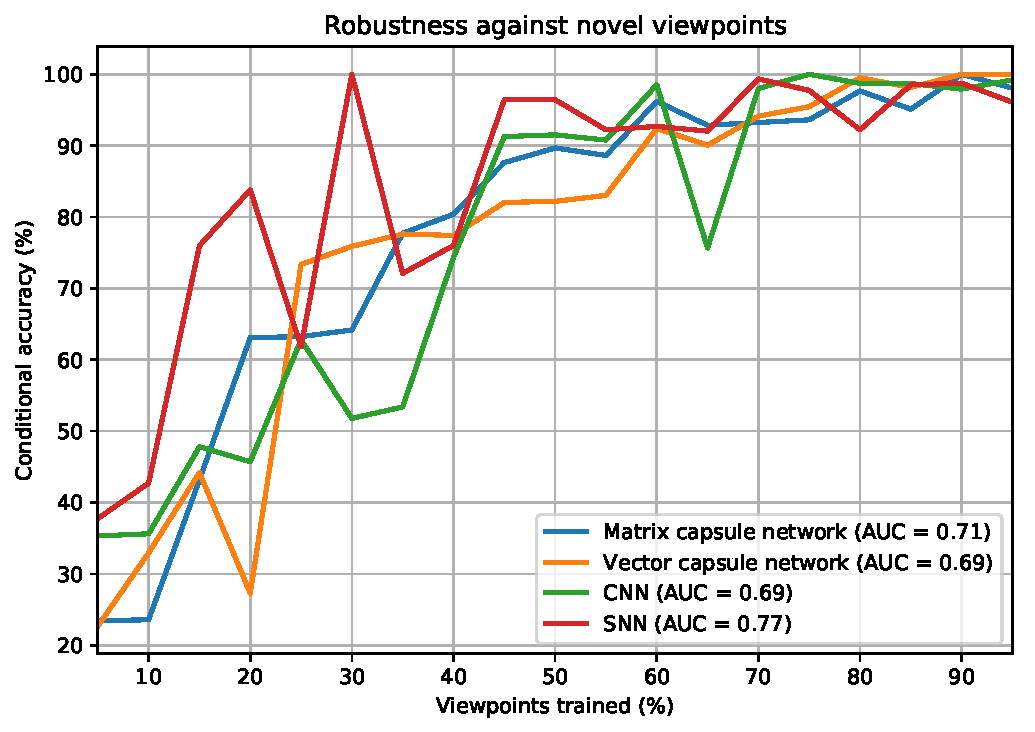
\includegraphics[width=\textwidth]{figures/viewpoints.pdf}
\caption[Generalization of the networks in the presence of untrained viewpoints]{Generalization of the networks in the presence of untrained viewpoints. There is quite a bit of fluctuation in the networks' conditional accuracy curve, whereas the matrix capsule's curve seems the most stable. The SNN particularly has a few spikes that give it the highest AUC. But other than that, no network is able to set itself apart. Note that as more viewpoints are included in the training, the more the curves converge to $\SI{100}{\percent}$, i.e. unperturbed performance.}\label{fig:viewpoint-generalization}
\end{figure}\noindent